
\chapter{Data and Model Distillation as a Solution for\\Domain-transferable Fact Verification \label{chapter:naacl21}}

\section{Introduction}

Neural networks have matched, and in several cases even surpassed, human performance in several supervised learning problems. However, such successes come at a cost. These neural networks typically need a great deal of human support in the form of man power required for curating domain specific datasets. Further, it has been shown \cite{gururangan-etal-2018-annotation, poliak-etal-2018-hypothesis,thorne2020avoiding} that several such models depend heavily on certain statistical nuances found in these datasets, information that transfers poorly between domains. The ideal solution to this problem is the creation of models that do not rely on such statistical nuances in the given datasets, but instead encode the true underlying semantics of the task, that are in turn transferable to other domains.



Fact verification is the task of verifying the truthfulness of claims by estimating their assertions against credible evidences. Specifically, given a pair of claim and evidence statements, they have to be classified into one of the 3 class labels, \textit{agree}, \textit{disagree}, or \textit{neutral}. Fact verification datasets, which often constitute real life news articles, have the added advantage of being used in practical problems such as fake news detection. More recently, several neural network models~\cite[inter alia]{nie-etal-2020-simple,liu-etal-2020-microsoft} built on top of the transformers \citep{vaswani2017attention}, have achieved excellent performance in fact verification tasks.

However these methods are not devoid of the shortcomings that besiege other neural networks in natural language processing tasks. It has been shown that these approaches depend heavily on lexical artifacts that transfer poorly between domains \cite{panenghat2020towards,karimi-mahabadi-etal-2020-end,schuster-etal-2019-towards}. For example, \citet{suntwal-etal-2019-importance} observed that out of all the statements containing the phrase `American Author' in  the FEVER dataset~\citep{thorne-etal-2018-fact}, 91\% of them belonged to one class label. Further, they demonstrated that neural methods put unnecessary emphasis on such lexical artifacts, which limits their transfer to other fact verification datasets such as the Fake News Challenge (FNC) \citep{pomerleau2017fake}.


To mitigate the dependency on such artifacts, \citet{suntwal-etal-2019-importance} proposed a {\em data distillation} (or delexicalization) approach, which replaces some lexical artifacts such as named entities with their type and a unique id to indicate occurrence of the same artifact in claim and evidence. While promising, the risk of this direction is discarding too much information through the delexicalization process. For example, replacing {\em China} with its named entity (NE) type ({\tt COUNTRY}) in an evidence sentence discards the fact that the text is about an Asian country which might be relevant in the context.

In this work we propose a solution that combines data distillation with {\em model distillation} to reduce the risk of over delexicalization. In particular, we introduce a teacher-student architecture inspired from that of \cite{tarvainen2017mean}. In our architecture, the student model is trained on delexicalized data (to take advantage of data distillation), but is also guided by a teacher trained on the original lexicalized data (as a form of model distillation) to mitigate the possibility of discarding too much lexical information. The contributions of our work are as follows:
{\flushleft {\bf (1)}} To our knowledge, we are the first to explore the combination of data and model distillation as a strategy to improve domain transfer of fact verification methods. Note that while our training process is more costly due to the combination of the student and teacher models, the output is a single individual model (the student), which has the same runtime cost as an individual classifier. Further, our approach is classifier agnostic, and can be coupled with any fact verification method.
{\flushleft {\bf (2)}} We investigate the domain transfer of our method between two fact verification tasks (FNC and FEVER), where we train on one and test on the other. For these experiments we couple our method with the state of the art fact verification approach based on transformers \citep{vaswani2017attention}. Our results indicate that our method achieves a cross-domain accuracy of 73.17\% in one of the experiments and 74.58\% in the other, outperforming other methods that do not use the data distillation-model distillation combination.

All the software for our proposed approach is open-source and publicly available on GitHub at: \url{https://github.com/clulab/releases/tree/master/naacl2021-student-teacher}.

\section{Methodology}

\subsection{Data distillation}

\citet{suntwal-etal-2019-importance} demonstrated that named entities are most prone to overfitting for fact verification.
Based on this observation, we also replace named entities with their type (and a unique id).
However, unlike their work, we have observed in early experiments that more fine-grained NE types yield better models. In particular, we utilize the FIGER  named entity recognizer (NER) \citep{ling2012fine} to detect and replace named entities with their most specific label returned by the NER. Further, we also process the text with the CoreNLP NER \citep{manning2014stanford} to delexicalize additional NER classes not covered by FIGER. We include in this list mentions of date, time, money, number, and ordinal.


\begin{table}[h]
% \begin{center}
\footnotesize
\begin{tabular}{p{10mm}p{26mm}p{30mm} }
\toprule
% \begin{tabular}{ p{0.\columnwidth}|p{0.4\columnwidth}|p{0.4\columnwidth} }
& \multicolumn{1}{c}{Claim} & \multicolumn{1}{c}{Evidence} \\
\midrule
\vspace{2mm}Plain text & \vspace{.1mm}Mark Zuckerberg made the Forbes list of The World's Most Powerful People  & In December 2016, Zuckerberg was ranked 10th on Forbes list of The World's Most Powerful People. \\
\midrule
\vspace{2mm}Distilled text & \vspace{.1mm}personC1 made the Forbes list of written\_workC1's Most Powerful People .   & In December 2016, personC1 was ranked 10th on Forbes list of written\_workC1 's Most Powerful People.  \\
\bottomrule
\end{tabular}
% \end{center}
\caption{  The claim and evidence before and after the data distillation process.}
\label{distillation_examples}
\end{table}


Next, we align the named entities between the claim and the evidence. That is, any named entity that appears first in the claim is assigned an id postfixed with \#C$n$; if an entity mention appears only in evidence then it is postfixed with \#E$n$, where C indicates that the entity appeared first in the claim, E indicates that the entity first appeared in the evidence, and $n$ indicates the $n$\textsubscript{th} observed entity. Table~\ref{distillation_examples} shows an example output for this data distillation process.

\subsection{Model distillation}


We propose a model distillation strategy to mitigate the risk of overly aggressive data distillation.
In particular, we introduce a  teacher-student architecture (shown in figure \ref{student_teacher_architecture}) \cite{hinton2015distilling,tarvainen2017mean,laine2016temporal,sajjadi2016regularization}, where the teacher is trained on the original, lexicalized data, and the student is trained on the data delexicalized with the approach described in the previous sub-section.


\begin{figure}[t!]
\center
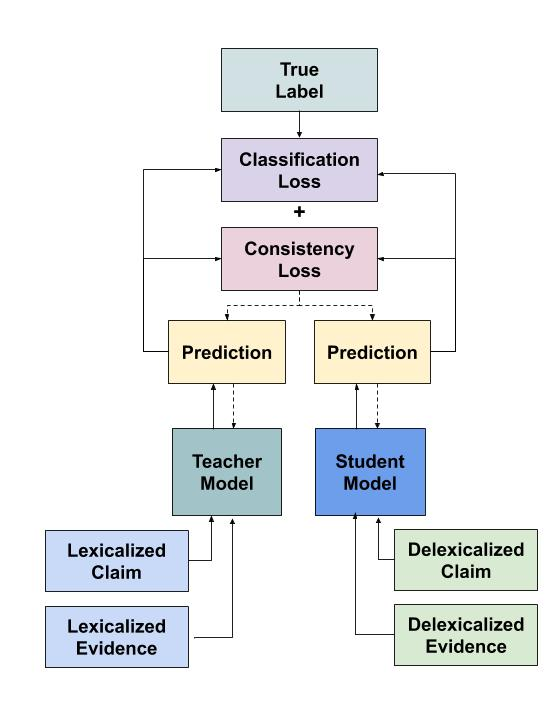
\includegraphics[width=0.9\linewidth]{mainmatter/naacl21_student_teacher/student_teacher_architecture_color_changed.jpeg}
\caption{ The teacher-student architecture for model distillation.}
\label{student_teacher_architecture}

\end{figure}

The intuition behind our model distillation approach is that the proposed teacher model will ``pull'' the student model towards the original underlying semantics, which are partially obscured to the student due to the delexicalization of its training data. More formally, this is captured through a consistency loss that minimizes the difference in predicted label distributions between the student and the teacher. The consistency loss is implemented as a mean squared error between the label scores predicted by the student and the teacher. Additionally, both the student and the teacher components include a regular classification loss on their respective data, which is implemented using cross entropy. This encourages both the student and the teacher to learn as much as possible from their own views of the data.



\subsection{Classifiers}

We experiment with a state-of-the-art method for fact verification, transformers \citep{vaswani2017attention}, which has achieved state-of-the-art results not only in the task of fact verification but in several other NLP tasks. Specifically, we use the PyTorch implementation of BERT \cite{devlin-etal-2019-bert} from huggingface \citep{wolf2019huggingface}.

We experimented with several pre-trained BERT-base models and found that the one which gave the highest performance was the BERT-cased model when used with a sequence length of 128. Further, to distinguish the vocabulary of the delexicalized data from the lexicalized data we augment the base vocabulary of BERT with tokens specific to the delexicalized data. For example, as mentioned before, during delexicalization we use \texttt{personC1} to denote the first occurence of the named entity in the claim paragraph. However, to ensure that the BERT BasicTokenizer does split \texttt{personC1} into \texttt{person}  and \texttt{C1}, we added the token ``C1'' to the BERT vocabulary. Tokenizers for each of the lexicalized and delexicalized dataset are initially created using BERT BasicTokenizer, but then use the aforementioned vocabulary created for the specific data type.




\begin{table*}[h!]
\begin{center}
\footnotesize
\begin{tabular}{p{40mm}p{9mm}p{9mm}p{9mm}p{9mm}}
\toprule
& \multicolumn{4}{c}{Configuration} \\
\midrule
Train Domain & {FEVER}&{FEVER}&{FNC}&{{FNC}} \\
Eval Domain & {FEVER}&{{FNC}}&{FNC}&{{FEVER}} \\
\midrule
BERT Lex&94.15\%&68.93\%&96.39\%&73.21\%\\
BERT Delex (OA-NER)&82.31\%&53.59\%&65.85\%&46.47\%\\
BERT Delex (OA-NER + SS)&75.26\%&46.71\%&45.51\%&51.77\%\\
BERT Delex (FIGER)&91.97\%&54.27\%&96.22\%&62.99\%\\
BERT TS (FIGER)&89.42\%&\textbf{73.14\%*}&98.89\%&\textbf{74.58\%*}\\
\bottomrule
\end{tabular}
\end{center}
\caption{\label{crossdomain} In-domain and cross-domain accuracies for various methods. All scores reported are averaged across three random seeds. ``BERT Lex'' is the stand alone model trained on the original lexicalized data; ``BERT Delex'' is the standalone model trained on delexicalized data. OA-NER delexicalizes the data using the Overlap Aware Named Entity Recognizer; SS uses Super Sense tags --- two  delexicalization techniques mentioned in \citet{suntwal-etal-2019-importance}. FIGER delexicalizes the data using a fine-grained named entity recognizer \citep{ling2012fine}. ; and ``BERT TS'' denotes the student in the proposed teacher-student architecture. * indicates that the corresponding result is significantly better than its baseline (``BERT lex'' in the same column), under a bootstrap resampling test with 1,000 samples, and $p$-value $<$ 0.035.
}
\label{results_fnc}

\end{table*}

\section{Experiments}

\subsection{Data}

We use two distinct fact verification datasets for
our experiments, FEVER \citep{thorne-etal-2018-fact} and FNC \citep{pomerleau2017fake}.

\textbf{The Fact Extraction and Verification (FEVER) dataset}: This dataset consists of 145,449 data points each having a claim and evidence pair. These claim-evidence pairs typically contain one or more sentences compiled from Wikipedia using an information retrieval (IR) module and are classified into three classes: \textit{supports, refutes} and \textit{not enough info}. The evidence for data points that had the gold label of \textit{not enough info} were  retrieved (using a task-provided IR component) either by finding the nearest neighbor to the claim or randomly. Even though the training partition of the FEVER dataset was publicly released, the gold test labels used in the final shared task were not. We therefore built our own test partition by dividing the randomized training partition into 80\% (119,197 data points) and 20\% (26,252 data points).

\textbf{The Fake News Challenge (FNC) dataset}: This dataset comprises claim-evidence pairs that were divided into four classes,
\textit{agree, disagree, discuss} and \textit{unrelated}. These claim-evidence pairs were created using the headlines and content section of real news articles respectively. While the training partition of the publicly available dataset comprised 49,972 data points, the testing partition had 25,413 data points. We further divided the training partition into
40,904 data points for training and 9,068 data points for development.

\textbf{Cross-domain labels:} In order to evaluate the proposed methods in a cross-domain setting, we modified the label space of the source domain to match that of the target domain. In particular, when training on FEVER and testing on FNC, the data points in FEVER that belong
to the class \textit{supports} were relabeled as \textit{agree}, and
those in \textit{refutes} as \textit{disagree}. Further, the data points belonging to the third class \textit{not enough info} (NEI) were divided into
\textit{discuss} and \textit{unrelated}. Specifically, of all the claim-evidence pairs that belonged to the NEI class, the ones whose evidences were retrieved using the nearest neighbor technique component of FEVER, were labeled to now belong to the \textit{discuss} class since they were more likely
to be topically relevant to the claim. The rest were assigned the label \textit{unrelated}. Similarly in the other direction, i.e., when training on FNC and testing on FEVER, the data points that had the labels of \textit{discuss} and \textit{unrelated} were combined and given the label of \textit{not enough info}.




\subsection{Settings}


In all the experiments, the performance of the underlying model on the respective lexicalized data is considered as the baseline. For example when training a teacher-student model on FEVER, the baseline is the model that was trained using the original text of the FEVER dataset. In the baseline model, we use the default hyper parameters set in the huggingface repository \citep{wolf2019huggingface}.


We focus our analysis on cross-domain evaluation, i.e., we train all models on one dataset  (e.g., FEVER) and evaluate their accuracy on the other dataset (e.g., FNC).



\subsection{Results}
Table \ref{results_fnc} summarizes the results of our experiments with various models tested in-domain and cross-domain. All scores reported are averaged across three random seeds. We use `BERT Lex' as the baseline model which is the stand alone model trained on the original lexicalized data. `BERT Delex' denotes the standalone models trained on delexicalized data, along with the corresponding delexicalization techniques used. OA-NER uses the Overlap Aware Named Entity Recognizer for delexicalization of data and SS uses Super Sense tags \citep{suntwal-etal-2019-importance}. FIGER delexicalizes the data using a fine-grained named entity recognizer \citep{ling2012fine}.  `BERT TS' denotes the student in the proposed teacher-student architecture.  Since the delexicalization used by the best performing `BERT Delex' models in the cross-domain setting was FIGER, we chose it as the preferred delexicalization technique for this student.

Note that the lexicalized models, which perform well in-domain, tend to transfer poorly to a new domain. For example, the BERT model trained
on lexicalized FEVER data, gave an accuracy of 94.15\% when tested on FEVER, but reduced to 68.93\% when tested on FNC.
This verifies our findings that the signal the model learns from unmasked text does not generalize well.

In contrast, in all our experiments, the student models trained under the teacher-student architecture outperform the other models trained using lexicalized data, in a cross-domain setting. For example, the student model of the teacher-student architecture trained on FEVER, gave an accuracy of 89.42\% when tested on FEVER and an accuracy of 73.14\% when tested on FNC. Similarly in the other direction, when the same model was trained on FNC, it gave an accuracy of 98.89\% when tested on FNC, and an accuracy of 74.58\% when tested on FEVER. Note that in both the directions the accuracy of the student model of the teacher-student architecture surpasses the corresponding accuracy of the model trained on lexicalized data in a cross-domain setting.
These experiments were repeated under a bootstrap resampling test with 1,000 samples, and $p$-value $<$ 0.035 to ensure statistical significance.




\subsection{Discussion}

We believe that the improved performance of the student model in the TS architecture is due to the fact that the TS architecture provides additional information over the ground labels. The key addition of our TS approach is that the delexicalized student learns to mimic the label probability distributions of the teacher through the consistency loss. As discussed earlier, we conjecture that this pulls the student model closer to the teacher. Another possible interpretation is that the model distillation has a regularization effect since the consistency loss essentially averages the behavior of both models.

Importantly, our results indicate that too much delexicalization risks discarding useful information. We believe this is why the standalone delexicalized model performs worse out of domain, and why the TS delexicalized student performs better.
Understanding {\em how much} delexicalization to apply given a task opens up interesting avenues for future research.
Nevertheless, overall this paper demonstrates that data distillation and model distillation can be combined as a strategy to improve domain transfer of fact verification methods.

\begin{table}[h]
\begin{center}
\begin{small}
\begin{tabular}{ c  |c }
Lex & TS Student \\
\hline
Apple&year\\
year& said\\
Rivers& {\tt country}\\
said& \texttt{person}\\
Islamic& according\\
State& \texttt{organization}\\
according& news\\
says& Islamic\\
Watch& \texttt{engineer}\\
report& \texttt{actor}\\

\end{tabular}
\end{small}
\end{center}
\caption{ Top 10 tokens with the highest attention weights by each of the trained models. `Lex' is the stand alone model trained on the original lexicalized data and `TS Student' denotes the student in the proposed teacher-student architecture.}
\label{attention_weights}

\end{table}

Lastly, we also inspected the word-level attention weights \citep{bahdanau2014neural} to further understand what these models are learning. Specifically, we analyze the weights assigned by the last attention head in the last layer of the respective transformer models. Table \ref{attention_weights} shows the tokens that were assigned highest weights by the model trained on lexicalized data and the teacher-student model.\footnote{Stop words and other BERT specific tokens like [SEP], [CLS], [PAD], etc., are removed from this list.} It can be seen that the tokens that were given the highest weights by the model trained on lexicalized data contain more named entities (e.g., {\em Apple}, {\em State}). This suggests potential overfitting, since the specific named entities should not be relevant for the fact verification task.

On the other hand, the tokens that were given the highest weights by the teacher-student model contain more generic named entity labels (e.g., country, person). Also we found that out of all the attention weights assigned by the model trained on lexicalized data, 15.60\% were given to named entities. Further, in the  TS student model only 7.44\% was assigned to named entity labels. These findings demonstrate that by using the data distillation and model distillation techniques we are able to reduce the importance that models place on lexical artifacts. This not only helps them achieve accuracies at par with their counterparts trained on plain text data in an
in-domain setting, but also outperform them in a cross-domain setting.

\section{Conclusion}
We present a new strategy to improve domain transfer of fact verification methods, which combines data distillation and model distillation.  We show that the performance of existing state-of-the-art models degrades significantly on a cross-domain setting,
hence motivating the
necessity of robust data distillation techniques such as delexicalization to minimize overfitting on lexical artifacts.
We further combine delexicalization with a teacher-student architecture as a form of model distillation to reduce the risk of over-delexicalization. We hope that this solution will encourage the development of architectures capable of reducing the dependency of models on lexical artifacts in an effort to learn domain transferable knowledge in the task
of fact verification.


\section*{Acknowledgments}

This work was supported by the Defense Advanced Research Projects Agency (DARPA) under the World Modelers program, grant number
W911NF1810014, and by the Bill and Melinda Gates Foundation HBGDki Initiative. Mihai Surdeanu declares a financial interest in lum.ai. This interest has been properly disclosed to the University of Arizona Institutional Review Committee and is managed in accordance with its conflict of interest policies. The authors would also like to thank Becky Sharp and Marco Valenzuela-Escárcega for all their valuable comments and reviews.










